\documentclass[11pt]{article}
% Shared preamble for the NSE working-paper series (Mrigank Sahi).
% Usage in each paper: % Shared preamble for the NSE working-paper series (Mrigank Sahi).
% Usage in each paper: % Shared preamble for the NSE working-paper series (Mrigank Sahi).
% Usage in each paper: \input{../common/preamble.tex}
\usepackage[T1]{fontenc}
\usepackage[utf8]{inputenc}
\usepackage{lmodern}
\usepackage{microtype}
\usepackage[a4paper,margin=1in]{geometry}
\usepackage{amsmath,amssymb}
\usepackage{booktabs}
\usepackage{tabularx}
\usepackage{siunitx}
\sisetup{group-separator={,},round-mode=places,round-precision=3}
\usepackage{graphicx}
\usepackage{xcolor}
\usepackage{caption}
\captionsetup{font=small,labelfont=bf}
\usepackage{enumitem}
\setlist{nosep,leftmargin=*}
\usepackage[framemethod=TikZ]{mdframed}
\usepackage[numbers,sort&compress]{natbib}
\usepackage[colorlinks=true,linkcolor=black,citecolor=blue!50!black,urlcolor=blue!50!black]{hyperref}

\newcommand{\ghbase}{https://github.com/mriganksahi-beep}
\newcommand{\authorline}{Mrigank Sahi\\\small Independent Researcher, New Delhi\\\small\texttt{mriganksahi@gmail.com}}

% Standard disclosure box. Every paper fills all five fields.
% #1 sample/period status, #2 position in test tally, #3 costs,
% #4 point-in-time limits, #5 anything else the reader must know
\newcommand{\caveatsbox}[5]{%
\begin{mdframed}[backgroundcolor=gray!8,linecolor=gray!50,innertopmargin=6pt,innerbottommargin=6pt]
\small\textbf{Read before interpreting results.}
\begin{itemize}
\item \textbf{Sample.} #1
\item \textbf{Multiple testing.} #2
\item \textbf{Costs.} #3
\item \textbf{Point-in-time universe.} #4
\item \textbf{Other.} #5
\end{itemize}
\end{mdframed}}

% Standard AI-assistance statement (identical across the series).
\newcommand{\aistatement}{%
\paragraph{Use of AI tools.} Code for this project was written with the assistance of
an AI coding assistant (Anthropic's Claude), working to specifications set by the
author, and the manuscript was drafted with the same assistance. The author designed
the research questions and decision rules and ran the main analyses. Some diagnostics
added during revision were computed by the assistant from archived run outputs; these
are labelled as revision diagnostics in the text. The author reviewed all code and
text and takes full responsibility for the content.}

% Standard data/code availability statement.
\newcommand{\availability}[1]{%
\paragraph{Data and code availability.} Code: \url{#1}. The point-in-time panel
construction is documented in \url{\ghbase/indian-equity-research/tree/main/data_pipeline}.
Price data from Yahoo Finance and index-membership snapshots from a licensed vendor
are not redistributed; the repository contains the scripts to rebuild the panel.}

% Placeholder for anything awaiting the author's confirmation. Renders red so it
% cannot survive into a posted PDF unnoticed.
\newcommand{\verify}[1]{\textcolor{red}{\textbf{[VERIFY: #1]}}}

\usepackage[T1]{fontenc}
\usepackage[utf8]{inputenc}
\usepackage{lmodern}
\usepackage{microtype}
\usepackage[a4paper,margin=1in]{geometry}
\usepackage{amsmath,amssymb}
\usepackage{booktabs}
\usepackage{tabularx}
\usepackage{siunitx}
\sisetup{group-separator={,},round-mode=places,round-precision=3}
\usepackage{graphicx}
\usepackage{xcolor}
\usepackage{caption}
\captionsetup{font=small,labelfont=bf}
\usepackage{enumitem}
\setlist{nosep,leftmargin=*}
\usepackage[framemethod=TikZ]{mdframed}
\usepackage[numbers,sort&compress]{natbib}
\usepackage[colorlinks=true,linkcolor=black,citecolor=blue!50!black,urlcolor=blue!50!black]{hyperref}

\newcommand{\ghbase}{https://github.com/mriganksahi-beep}
\newcommand{\authorline}{Mrigank Sahi\\\small Independent Researcher, New Delhi\\\small\texttt{mriganksahi@gmail.com}}

% Standard disclosure box. Every paper fills all five fields.
% #1 sample/period status, #2 position in test tally, #3 costs,
% #4 point-in-time limits, #5 anything else the reader must know
\newcommand{\caveatsbox}[5]{%
\begin{mdframed}[backgroundcolor=gray!8,linecolor=gray!50,innertopmargin=6pt,innerbottommargin=6pt]
\small\textbf{Read before interpreting results.}
\begin{itemize}
\item \textbf{Sample.} #1
\item \textbf{Multiple testing.} #2
\item \textbf{Costs.} #3
\item \textbf{Point-in-time universe.} #4
\item \textbf{Other.} #5
\end{itemize}
\end{mdframed}}

% Standard AI-assistance statement (identical across the series).
\newcommand{\aistatement}{%
\paragraph{Use of AI tools.} Code for this project was written with the assistance of
an AI coding assistant (Anthropic's Claude), working to specifications set by the
author, and the manuscript was drafted with the same assistance. The author designed
the research questions and decision rules and ran the main analyses. Some diagnostics
added during revision were computed by the assistant from archived run outputs; these
are labelled as revision diagnostics in the text. The author reviewed all code and
text and takes full responsibility for the content.}

% Standard data/code availability statement.
\newcommand{\availability}[1]{%
\paragraph{Data and code availability.} Code: \url{#1}. The point-in-time panel
construction is documented in \url{\ghbase/indian-equity-research/tree/main/data_pipeline}.
Price data from Yahoo Finance and index-membership snapshots from a licensed vendor
are not redistributed; the repository contains the scripts to rebuild the panel.}

% Placeholder for anything awaiting the author's confirmation. Renders red so it
% cannot survive into a posted PDF unnoticed.
\newcommand{\verify}[1]{\textcolor{red}{\textbf{[VERIFY: #1]}}}

\usepackage[T1]{fontenc}
\usepackage[utf8]{inputenc}
\usepackage{lmodern}
\usepackage{microtype}
\usepackage[a4paper,margin=1in]{geometry}
\usepackage{amsmath,amssymb}
\usepackage{booktabs}
\usepackage{tabularx}
\usepackage{siunitx}
\sisetup{group-separator={,},round-mode=places,round-precision=3}
\usepackage{graphicx}
\usepackage{xcolor}
\usepackage{caption}
\captionsetup{font=small,labelfont=bf}
\usepackage{enumitem}
\setlist{nosep,leftmargin=*}
\usepackage[framemethod=TikZ]{mdframed}
\usepackage[numbers,sort&compress]{natbib}
\usepackage[colorlinks=true,linkcolor=black,citecolor=blue!50!black,urlcolor=blue!50!black]{hyperref}

\newcommand{\ghbase}{https://github.com/mriganksahi-beep}
\newcommand{\authorline}{Mrigank Sahi\\\small Independent Researcher, New Delhi\\\small\texttt{mriganksahi@gmail.com}}

% Standard disclosure box. Every paper fills all five fields.
% #1 sample/period status, #2 position in test tally, #3 costs,
% #4 point-in-time limits, #5 anything else the reader must know
\newcommand{\caveatsbox}[5]{%
\begin{mdframed}[backgroundcolor=gray!8,linecolor=gray!50,innertopmargin=6pt,innerbottommargin=6pt]
\small\textbf{Read before interpreting results.}
\begin{itemize}
\item \textbf{Sample.} #1
\item \textbf{Multiple testing.} #2
\item \textbf{Costs.} #3
\item \textbf{Point-in-time universe.} #4
\item \textbf{Other.} #5
\end{itemize}
\end{mdframed}}

% Standard AI-assistance statement (identical across the series).
\newcommand{\aistatement}{%
\paragraph{Use of AI tools.} Code for this project was written with the assistance of
an AI coding assistant (Anthropic's Claude), working to specifications set by the
author, and the manuscript was drafted with the same assistance. The author designed
the research questions and decision rules and ran the main analyses. Some diagnostics
added during revision were computed by the assistant from archived run outputs; these
are labelled as revision diagnostics in the text. The author reviewed all code and
text and takes full responsibility for the content.}

% Standard data/code availability statement.
\newcommand{\availability}[1]{%
\paragraph{Data and code availability.} Code: \url{#1}. The point-in-time panel
construction is documented in \url{\ghbase/indian-equity-research/tree/main/data_pipeline}.
Price data from Yahoo Finance and index-membership snapshots from a licensed vendor
are not redistributed; the repository contains the scripts to rebuild the panel.}

% Placeholder for anything awaiting the author's confirmation. Renders red so it
% cannot survive into a posted PDF unnoticed.
\newcommand{\verify}[1]{\textcolor{red}{\textbf{[VERIFY: #1]}}}

\usepackage{xurl} % allow line breaks anywhere in long repository URLs

\title{Momentum in the Nifty 500: What Survives in Liquid Names,\\
and Six Enhancement Tests That Did Not Pass Their Decision Rules}
\author{\authorline}
\date{October 2026}

\begin{document}
\maketitle

\begin{abstract}
\noindent On a snapshot-based point-in-time Nifty 500 universe, the equal-weighted 12-1
momentum decile spread (D10$-$D1) averages 1.74\% per month. Its annualised Sharpe ratio
is 0.85, with a 95\% block-bootstrap interval of 0.34 to 1.50. These figures are gross of
costs and cover 179 monthly rebalances from 2011 to 2026, a span that includes the period
later designated as hold-out. The main test rebuilt the deciles inside the most liquid
30, 50 and 70\% of names. No liquidity floor passed the registered joint screen (interval
lower bound above 0.30 and decile monotonicity above 0.5), and the full universe did not
pass either. Point estimates stay positive at every floor but decline as the universe
narrows. Six enhancement and diagnostic hypotheses were not supported
under their own decision rules, and three of them are inconclusive rather than negative.
The results are historical, gross-of-cost evidence, not a validated investable strategy.
\end{abstract}

\caveatsbox{%
All results use the full sample: rebalances 2011-01-31 to 2026-06-30, with returns
through 2026-07-10. That includes 2022 onward, the period the project later reserved as
a hold-out. The baseline ran before the hold-out rule existed. The enhancement batch and
the liquidity test also report full-sample results, and M1 and M3 additionally looked
once at a 2011--2021 vs.\ 2022--2026 split. No result here is a clean out-of-sample test.}{%
In the legacy project ledger, the enhancement batch holds sub-tests 1--29: M1 1--9,
M3 10--14, M4 15--18, M5 19--24, M6 25--28 and M7 29. No M2 exists in the archived
sequence. The ledger reached 32 with tests outside this paper. The baseline (MOM-B) and
the liquidity-universe test (MOM-L) sit outside the legacy count. Provisional Deflated
Sharpe Ratios were computed at 6 and 14 trials; they are not relied on here.}{%
Every return is gross of brokerage, taxes, bid-ask spreads and market impact. The one
exception is M1, which applies a simplified capital-gains tax to the long leg only. No
result is net of trading costs, and no capacity analysis was done.}{%
Membership is a snapshot-based approximation built from 33 semi-annual index snapshots,
so a stock's status can be up to about six months off. The 2018-06-30 snapshot is
truncated, which may misclassify up to about 22\% of names in July--December 2018.
Eligibility also requires a complete trailing-year return window, so the tested universe
is not the whole index.}{%
Seven mid-sample month-ends were dropped. Most fell on dates the panel lists although
the exchange was closed. A calendar-corrected rerun is pending and could change every
number in this paper. Intervals are 95\% percentile block-bootstrap intervals (12-month
blocks, 10,000 resamples): circular for the baseline, non-circular moving-block for the
liquidity and M5 analyses. The other batch statistics are $t$-statistics or point
estimates. Analyses added during drafting are labelled \emph{post hoc}.}

\section{Introduction}

Momentum is one of the best-documented cross-sectional return patterns
\citep{jegadeesh1993,asness2013}, and it is prone to crashes \citep{daniel2016,barroso2015}.
This paper does not claim to discover momentum in India. It contributes a careful
implementation on a snapshot-based Nifty 500 universe, organised around one practical
question: \emph{how much of the 12-1 momentum spread remains when the portfolio is built
only from more liquid names?} That question matters because the baseline effect is
strongest in the least-traded stocks. Two smaller contributions accompany it. The first
is the baseline estimate with its uncertainty. The second is a record of six
pre-registered refinements and diagnostics (M1, M3--M7) that did not pass their own
criteria.

\paragraph{Summary of findings.} The full-sample, gross baseline spread is positive, and
its block-bootstrap interval excludes zero. The decile profile is broadly ordered: 7 of 9
adjacent steps rise. When deciles are rebuilt inside liquid subsets, point estimates
remain positive. The Sharpe ratio falls from 0.755 (full universe, same harness) to
0.710, 0.507 and 0.394 at the top 70, 50 and 30\% by turnover. No floor met the
registered joint screen, so the liquidity result is suggestive, not decision-grade. None
of the batch hypotheses was supported. Regime-conditional momentum is covered in
\citet{sahi_irfa}, and path entropy (M7) in \citet{sahi_pathtexture}.

\section{Data and universe}

The panel is a daily feature panel: 3,328,132 rows, 4,237 dates and 1,069 tickers, from
2010-01-04 to 2026-07-10. Prices come from Yahoo Finance, with Bloomberg filling 114
tickers; the Yahoo close is split-adjusted. Construction is documented in
\url{\ghbase/indian-equity-research/tree/main/data_pipeline}. Membership is a tri-state daily flag expanded from 33
semi-annual snapshots, and every test uses \texttt{flag == 1}.

Choices specific to this paper:
\begin{itemize}
\item \textbf{Rebalance dates.} The rebalance date is the panel's last date in each
calendar month, which yields 199 month-ends. Months with fewer than 100 eligible names
are dropped. That removes 12 in 2010 (warm-up) and 7 mid-sample: 2011-08-31,
2014-08-29, 2015-02-28, 2016-10-31, 2018-03-29, 2019-03-29 and 2020-11-30. Five of the
seven coincide with exchange holidays on which the panel carried incomplete rows. The
panel's date index contains such closed dates, so the cross-section collapses on them.
2015-02-28 was a genuine special Saturday session held for the Union Budget, with few
rows in the panel. 2019-03-29 is unexplained.
\item \textbf{Eligibility.} The 232 trading rows $[t-252,\,t-21]$ (inclusive) must all
have valid returns. The one vendor-failure date (2025-03-18) and the row after it are
excused, so the requirement becomes $232$ minus the number of excused rows. Average
eligible names by year range from 411 (2024) to 492.
\item \textbf{Corporate actions.} Eight tickers with unadjusted split splices are
removed from return paths in the batch and liquidity harnesses, but not in the Phase B
baseline.
\item \textbf{Liquidity.} Turnover is the mean of daily volume times close over rows
$[t-21,\,t-1]$, with at least 15 valid values. Amihud illiquidity \citep{amihud2002} is
taken from a monthly file and lagged one month.
\end{itemize}

\section{Method}

\paragraph{Signal and portfolios.} For stock $i$ at rebalance $t$, the momentum signal is
$m_{i,t}=\prod_{s=t-252}^{t-21}(1+r_{i,s})-1$ over trading rows. Eligible names are
ranked each month; ties go to the first name in ticker order. Decile assignment is
$\lceil 10\,\mathrm{rank}/N_t\rceil$. The monthly spread is
$S_t=\bar R_{D10,t}-\bar R_{D1,t}$ (equal-weighted), and the Sharpe ratio is
$\sqrt{12}\,\bar S/\hat\sigma_S$. Inference treats the monthly spread series as the unit.
Twelve-month blocks preserve autocorrelation at up to a year, which suits a signal with a
twelve-month memory.

\paragraph{Liquidity-universe test (MOM-L, main analysis).} Each month the test keeps
the top 30, 50 or 70\% of eligible names by trailing turnover (primary measure) or by
lowest prior-month Amihud (robustness). It then forms new momentum deciles inside that
subset and computes D10$-$D1. The floors, the headline statistic and the joint screen
were fixed before the run: Sharpe interval lower bound $>0.30$ \emph{and} Spearman
monotonicity of the time-averaged decile profile $>0.5$. The full curve is reported.

\paragraph{Enhancement batch (M1, M3--M7).} Each mechanism had a registered headline
statistic and decision rule, and each ran against the frozen signal. The rules are
summarised in Table~\ref{tab:mbatch}. Regression-based tests use Fama--MacBeth
coefficients \citep{fama1973}, with Newey--West standard errors at six lags
\citep{newey1987} where the source says so.

\paragraph{Harnesses.} The three notebooks implement the ``same'' strategy differently
(Table~\ref{tab:harness}). For that reason every comparison in this paper is made within
a single harness.

\begin{table}[t]
\centering\footnotesize
\caption{Implementation harnesses. All are equal-weighted, use the 12-1 signal with the
232-row window, require at least 100 names, and are gross of costs.}
\label{tab:harness}
\begin{tabularx}{\linewidth}{@{}l>{\raggedright\arraybackslash}X>{\raggedright\arraybackslash}X>{\raggedright\arraybackslash}X@{}}
\toprule
& Phase B baseline (MOM-B) & Liquidity test (MOM-L) & M1/M3 batch harness \\
\midrule
Dates & Rebalances 2011-01-31 to 2026-06-30 & Same span & Windows ending 2011-02-28 to 2026-07-10 \\
Months & 179 (7 mid-sample skips) & 179 & 186 (no gaps; see Section~\ref{sec:robust}) \\
Forward return & Compounded over the stock's rows in (rebalance, next month-end] & Next 21 trading rows of that stock & Monthly mark-to-market of the held book \\
Missing forward return & Observed days compounded; the 9 positions with none excluded & Name excluded & Weights renormalised over names with a return \\
Corporate-action screen & No & Yes (8 tickers) & Yes (8 tickers) \\
Bootstrap & Circular block, 12 months, 10,000 draws, seed 20260724 & Moving block (non-circular), 12 months, 10,000 draws, same seed & None for M1/M3 headline \\
Full-universe Sharpe & 0.847 & 0.755 & 0.910 (M1); 0.859 (M3, volatility-matched) \\
\bottomrule
\end{tabularx}
\end{table}

\paragraph{Validation gates actually run.}
\begin{itemize}
\item \textbf{Leakage.} No signal window, out of 133,281, ended on or after its
rebalance; the smallest gap was 28 calendar days. Turnover windows ended before the
rebalance date. The M4 test checked that its signal, gate and forward windows meet
without overlapping.
\item \textbf{Spot-checks.} A hand computation matched the vectorised signal exactly
for GIPCL (2011-12-30), MOTHERSON (2019-06-28) and JISLJALEQS (2025-07-31).
\item \textbf{PIT universe.} The flag drops RANBAXY and HDFC after their mergers (0 of 8
and 0 of 9 later months flagged in). The eligible count varies across dates (standard
deviation 139.6), so the filter is live.
\item \textbf{Exits.} Only 37 positions ended because the stock stopped trading (0.043\%
of eligible stock-months), spread evenly across deciles.
\item \textbf{Detection power.} Synthetic data with a planted signal confirmed the tests
can find a real effect. M4's regression recovered a planted interaction of $+0.8$ as
0.801, and M6's Lind--Mehlum test found a planted hump and rejected a monotonic-concave
curve.
\item \textbf{Post hoc reproduction.} \texttt{make\_figures.py} recomputes the decile
means, the spread, the Sharpe ratio and its bootstrap interval from the archived baseline
CSVs, and checks that they match the notebook output exactly.
\end{itemize}

\section{Results}

\subsection{Baseline (MOM-B)}

Table~\ref{tab:baseline} and Figure~\ref{fig:staircase} report the baseline. The spread
interval and the IC interval both exclude zero. Decile means rise from 0.22\% to 1.96\%
per month, but D5 is below D4 and D9 is below D8. The two end steps contribute 1.05 of
the 1.74 percentage points. Figure~\ref{fig:cum} shows losing years in 2020 (the
expected momentum crash, a 46.7\% drawdown between January and September), 2024 and the
first half of 2026.

The mutual-information study \citep{sahi_mi} reports a momentum IC of 0.085 for
2010--2021 and 0.084 for 2011--2021 in its own harness. The start date therefore does
not explain the gap with the 0.0605 reported here. The gap comes from including
2022--2026, from harness differences, or both, and has not been decomposed.

\begin{table}[t]
\centering\small
\caption{Phase B baseline: D10$-$D1, equal-weighted, gross of costs, full sample of 179
rebalances. Intervals are 95\% percentile intervals from a circular block bootstrap
(12-month blocks, 10,000 resamples). Terciles are slices of the full-universe deciles by
turnover, specific to this harness.}
\label{tab:baseline}
\begin{tabular}{lrl}
\toprule
Statistic & Estimate & 95\% interval \\
\midrule
Mean spread (\% per month) & 1.740 & [0.769, 2.705] \\
Annualised Sharpe ratio ($\sqrt{12}$ convention) & 0.847 & [0.335, 1.503] \\
Annualised return / volatility (\%) & 19.1 / 24.7 & -- \\
Months with positive spread (\%) & 64.8 & -- \\
Mean monthly Spearman IC; months with IC $>0$ (\%) & 0.0605; 66.5 & [0.0350, 0.0865] \\
Adjacent decile steps that rise & 7 of 9 & -- \\
Worst month; Jan--Sep 2020 maximum drawdown (\%) & $-37.3$; $-46.7$ & -- \\
Tercile Sharpe ratios: illiquid / middle / liquid & 0.88 / 0.95 / 0.42 & -- \\
\bottomrule
\end{tabular}
\end{table}

\begin{figure}[t]
\centering
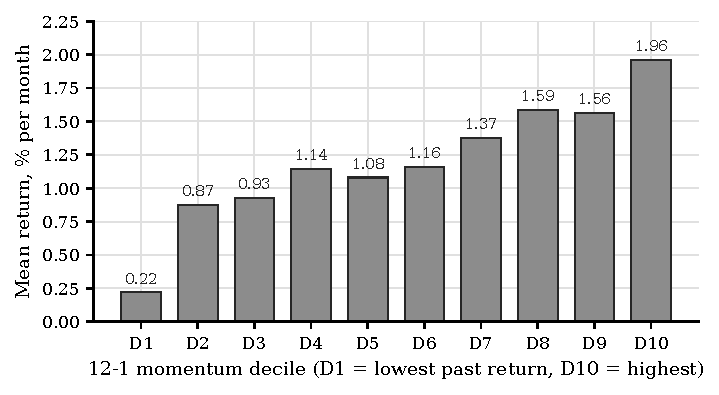
\includegraphics[width=0.74\linewidth]{figures/fig1_decile_staircase.pdf}
\caption{Mean equal-weighted monthly return by 12-1 momentum decile. Phase B baseline,
full sample (179 months), gross of costs. Seven of nine adjacent steps rise.}
\label{fig:staircase}
\end{figure}

\begin{figure}[t]
\centering
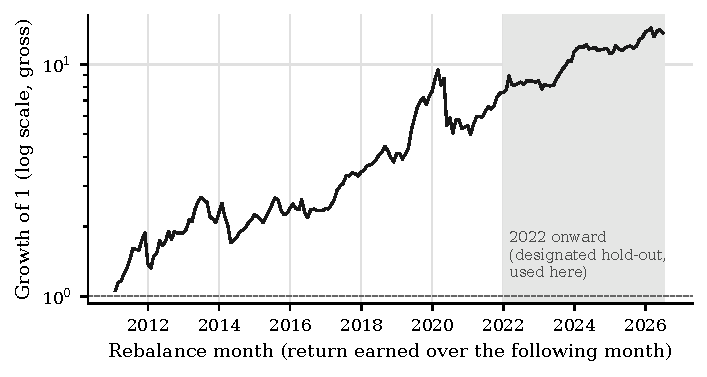
\includegraphics[width=0.74\linewidth]{figures/fig3_cumulative_spread.pdf}
\caption{Cumulative D10$-$D1 spread on a log scale, gross of costs. The shaded area is the
period the project later designated as hold-out. This baseline used it, so the figure is
not out-of-sample evidence.}
\label{fig:cum}
\end{figure}

\subsection{Liquidity-universe test (MOM-L)}

Table~\ref{tab:liquid} and Figure~\ref{fig:liquid} report the main analysis. All eight
filtered runs fail the registered joint screen (four floors under each of two liquidity
measures). Every run, including the full universe, fails on the interval criterion,
while all pass on monotonicity. Point estimates decline as the universe narrows, and the
two liquidity measures agree to within 0.09 at every floor. At the top 70\%, both
intervals exclude zero. At the top 50\%, the turnover interval only just excludes zero
and the Amihud interval includes it. At the top 30\%, both include zero. Intervals for
different floors overlap, so the ordering across floors is a central tendency, not an
established difference.

As a \emph{post hoc} point-estimate description, the floor Sharpe ratios are 94\%
(turnover) and 82\% (Amihud) of the same-harness full-universe value at the top 70\%,
and 67--68\% at the top 50\%. These ratios have no interval, were chosen after the
results were seen, and are not evidence that liquid momentum is investable. The top-30\%
rebuilt universe (0.394) and the Phase B liquid tercile (0.42) are close, and they come
from different harnesses. The data therefore do not support the claim that rebuilding
deciles, as opposed to slicing them, changes the liquid-name result.

\begin{table}[t]
\centering\small
\caption{Liquidity-universe test (MOM-L): deciles rebuilt within each floor, D10$-$D1,
equal-weighted, gross, full sample, 179 months. Intervals are 95\% percentile intervals
from a moving-block bootstrap (12-month blocks, 10,000 resamples). Mono.\ is the Spearman
correlation of the decile profile with decile number. The screen requires an interval
lower bound above 0.30 \emph{and} Mono.\ above 0.5. Ret.\ (post hoc) is the floor Sharpe
divided by the full-universe Sharpe, a ratio of point estimates.}
\label{tab:liquid}
\setlength{\tabcolsep}{3.2pt}
\begin{tabular}{lrrlrrrlrrc}
\toprule
& & \multicolumn{4}{c}{Turnover filter (primary)} & \multicolumn{4}{c}{Amihud filter (robustness)} & \\
\cmidrule(lr){3-6}\cmidrule(lr){7-10}
Floor & Names & Sharpe & 95\% interval & Mono. & Ret. & Sharpe & 95\% interval & Mono. & Ret. & Screen \\
\midrule
Top 30\% & 143 & 0.394 & [$-$0.111, 0.789] & 0.75 & 52\% & 0.394 & [$-$0.089, 0.856] & 0.79 & 52\% & fail/fail \\
Top 50\% & 238 & 0.507 & [0.016, 0.922] & 0.87 & 67\% & 0.519 & [$-$0.012, 0.991] & 0.84 & 68\% & fail/fail \\
Top 70\% & 332 & 0.710 & [0.182, 1.157] & 0.98 & 94\% & 0.622 & [0.051, 1.123] & 0.98 & 82\% & fail/fail \\
Full & 475 & 0.755 & [0.186, 1.323] & 0.94 & -- & 0.758 & [0.190, 1.326] & 0.94 & -- & fail/fail \\
\midrule
\multicolumn{11}{l}{Mean spread, \% per month. Turnover: 0.96, 1.09, 1.44, 1.54. Amihud: 0.90, 1.11, 1.25, 1.54.}\\
\bottomrule
\end{tabular}
\end{table}

\begin{figure}[t]
\centering
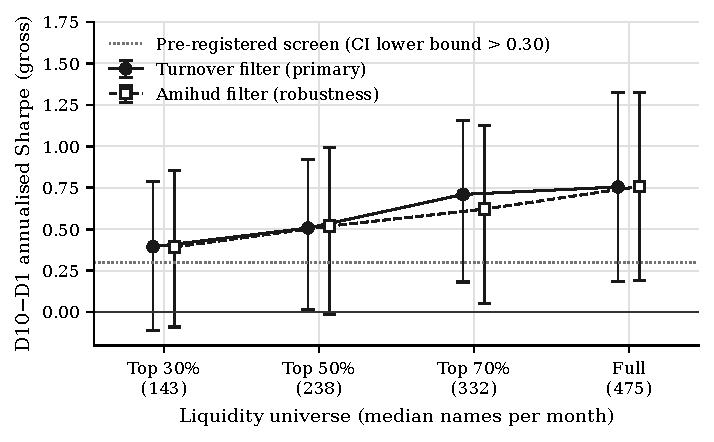
\includegraphics[width=0.74\linewidth]{figures/fig2_liquidity_retention.pdf}
\caption{D10$-$D1 Sharpe ratio with deciles rebuilt within each liquidity universe, with
95\% moving-block bootstrap intervals. Full sample, gross of costs. No floor's interval
lower bound clears the registered 0.30 screen (dotted line).}
\label{fig:liquid}
\end{figure}

\subsection{Enhancement batch}

\begin{table}[t]
\centering\footnotesize
\caption{Registered enhancement and diagnostic hypotheses. All are full sample and
gross of transaction costs. ``Reading'' applies the registered rule. A result is
``inconclusive'' when its interval, or its $t$ against the bar, does not exclude zero.}
\label{tab:mbatch}
\begin{tabularx}{\linewidth}{@{}l>{\raggedright\arraybackslash}X>{\raggedright\arraybackslash}X>{\raggedright\arraybackslash}p{2.3cm}@{}}
\toprule
& Registered claim and rule & Headline evidence & Reading \\
\midrule
M1 & Rebalancing every 2, 3 or 6 months, or hysteresis bands, keeps $\geq$90\% of gross Sharpe \emph{and} materially cuts after-tax drag &
Quarterly: 99.9\% of 0.910, after-tax change $+0.02$\% per month; semiannual: 69.8\%, $-0.54$\%; bands 78--90\%, all after-tax changes negative &
Not supported (point estimates; no intervals) \\
M3 & Volatility-scaled ranking narrows the illiquid-minus-liquid tercile Sharpe gap &
Gap 0.277 (plain) $\to$ 0.581 (vol-120) and 0.360 (vol-60), in M3's 186-month harness &
Not supported; moved the opposite way (no interval on the gap) \\
M4 & The skipped-month return gates momentum: Fama--MacBeth interaction, Newey--West $t>2$ &
Interaction 0.00107, $t=1.91$; 1 of 4 gate forms reached $t=2.04$ &
Inconclusive under the registered threshold \\
M5 & Younger trends outperform after removing momentum (primary proxy: 52-week high) &
Young minus mature $-0.021$\% per month, iid $t=-0.05$, moving-block 95\% interval [$-0.64$, $+0.65$] &
Inconclusive \\
M6 & The mid-liquidity Sharpe peak is a genuine interior maximum (Lind--Mehlum) &
0 of 4 curves (Amihud, turnover $\times$ 10 and 20 buckets) pass &
Not supported \\
M7 & Smooth (low-entropy) paths outperform at equal momentum (distinctness gate) &
Entropy coefficient Newey--West $t=-0.29$; later gates not reached &
Inconclusive; see \citet{sahi_pathtexture} \\
\bottomrule
\end{tabularx}
\end{table}

Table~\ref{tab:mbatch} summarises the batch. The notes below record what each test
actually computed, and separate headline results from supporting cuts.

\textbf{M1} tracked tax lots first-in-first-out and taxed the long leg at 20\% if a lot
was held 365 days or less, 12.5\% otherwise. Those are the rates in force since July
2024, and the model applied them across the whole sample. It had no exemption, no loss
harvesting, an assumed capital of Rs 1 crore and a gross short leg, so it is not a
historical tax calculation. Quarterly rebalancing kept the gross Sharpe but left 91\% of
exits short-term. In this model the 365-day threshold, not turnover, was the binding
constraint.

\textbf{M3}'s linear Fama--MacBeth liquidity controls left the momentum coefficient
intact (104\%). That reflects a specification limitation, not evidence that the effect
is independent of liquidity. The explicit signal-by-illiquid interaction ($t=1.75$) is
suggestive only.

\textbf{M4}: the supporting cuts do not establish an effect (sign-only $t=0.54$, 63-day
horizon $t=0.80$, no liquidity tercile above $t=1.4$). The single form at $t=2.04$ is one
of four examined.

\textbf{M5}'s secondary golden-cross proxy gave $+0.401$\% per month. Its iid
$t$-statistic is 1.68, computed as the mean over its standard error, not Newey--West. Its
moving-block bootstrap interval of [$+0.08$, $+0.71$] excludes zero. The two methods
disagree, so this is an exploratory secondary result, not a pass; the registered primary
proxy did not pass. On crash risk, young trends had deeper maximum drawdowns than mature
ones under all three proxies, including after scaling by volatility. The frequency of
months below $-10$\% was higher for young trends only under the 52-week-high proxy (8.4\%
vs.\ 1.7\%). Under the 200-day moving average it was lower (2.6\% vs.\ 3.8\%), and under
golden-cross age it was equal (3.2\%).

\textbf{M6}: with finer buckets the momentum coefficient rises toward illiquid names on
Amihud (0.0017 to 0.0091) and falls toward high-turnover names (0.0113 to 0.0011). The
interpretation best supported by the Lind--Mehlum tests \citep{lind2010} is that the
three-bucket ``hump'' arose from coarse bucketing of a roughly monotonic gradient.

\textbf{M7} is reported in \citet{sahi_pathtexture}. The permutation entropy
\citep{bandt2002} of formation-window daily returns showed no relation to forward returns
($t=-0.29$, and $-0.12$ after controlling for frog-in-the-pan, \citealp{da2014}).
Entropy values fell in a narrow 0.95--1.0 band, and the gate design stopped the test
before any performance number was computed.

Two by-products were never registered as hypotheses: a constant-volatility overlay
\citep{barroso2015}, with Sharpe 0.899 vs.\ 0.859, and signal-proportional weighting,
with 0.898 vs.\ 0.767 equal-weight within the (10,8) band. Both are exploratory and would
need a new, frozen test.

\section{Robustness and diagnostics}\label{sec:robust}

\paragraph{179 vs.\ 186 months (post hoc reconciliation).} The M1 notebook attributes
its seven extra months to a forward-return convention that reached later dates. The
archived counts do not support that explanation. M1 splits its 186 months into 131 that
end before 2022 and 55 that end on or after it. Those are exactly the number of calendar
months from 2011-02 to 2021-12 and from 2022-01 to 2026-07, so M1 has no gaps and
shares Phase B's first and last windows. Phase B has 124 and 55 under the same split.
All seven extra M1 observations are therefore the seven interior months Phase B skipped.
M1's code keeps the previous month's book and marks it to market through them
(\texttt{reconcile\_months.py}).

\paragraph{Liquidity measures.} Turnover and Amihud give the same ordering. In M6 the
two measures slope in opposite directions by construction while reaching the same
economic conclusion.

\paragraph{2018 window and coverage.} The mean spread over July--December 2018 was
0.462\% per month ($n=6$), against 1.784\% in the other months (rough $z=0.45$).
Dropping that window did not change M6. Of all (ticker, rebalance) pairs, 62.65\% have a
valid signal. A looser 186-of-232-row rule would add 3.66 percentage points. In 2024 the
strict window removed 18.3\% of names that had a full window, against 3.9--17.9\% in
other years. The filter responsible has not been audited.

\section{Limitations and what this paper does not establish}

\begin{itemize}
\item \textbf{No untouched hold-out.} A test on data after July 2026, under a frozen
protocol, would be needed.
\item \textbf{Calendar defect.} Seven months were lost to closed or thin dates, and a
closed date inside a window shifts row-counted windows by a day. The calendar-fix rerun
is pending.
\item \textbf{Harness differences.} No common-harness baseline exists. The cross-harness
Sharpe range of 0.755--0.910 is an implementation effect of about the same size as some
of the comparisons of interest.
\item \textbf{Investability.} There is no cost model, no capacity analysis, and no
per-floor turnover, holding count or concentration. Delisting proceeds are not modelled:
Phase B compounds a stopped stock's observed days, and the liquidity harness drops names
with no forward rows. Equal weighting tilts toward the smallest names in each universe.
\item \textbf{Precision.} Even the full-universe Sharpe interval spans 0.19--1.32.
\end{itemize}

\noindent\textbf{What this paper does not establish.} It does not show that liquid-name
momentum is investable or profitable after costs. It does not show that any liquidity
floor beats any other. It does not show that the six refinements have zero effect: three
are inconclusive. It does not show that the exploratory by-products work. And it offers
no out-of-sample validation of any result.

\section{Conclusion}
Across the historical sample, the equal-weighted 12-1 momentum decile spread is positive,
and its block-bootstrap interval excludes zero. The decile profile is broadly ordered
rather than strictly monotonic. When deciles are rebuilt inside more liquid subsets, the
point estimates remain positive. Uncertainty is wide, though, and none of the
pre-specified liquidity floors passed the joint screen. The results include the later
hold-out period, rely on different implementation harnesses and are gross of trading
costs, so they are historical evidence rather than a validated investable strategy. The
registered enhancement hypotheses were not supported under their stated decision rules,
and the exploratory variants would need a new, frozen test.

\begin{table}[h]
\centering\footnotesize
\caption{Reproducibility. Colab software versions were not recorded. The post hoc
reproduction used Python 3.13, NumPy 2.5.3, pandas 3.0.5 and Matplotlib 3.11.2.}
\label{tab:repro}
\begin{tabularx}{\linewidth}{@{}l>{\raggedright\arraybackslash}X@{}}
\toprule
Item & Value \\
\midrule
Panel & \texttt{feature\_panel\_with\_pit\_v2\_2026-07-24.parquet} (3,328,132 rows); Amihud \texttt{amihud\_monthly\_v2\_2026-07-24.parquet} \\
MOM-B & Run 2026-07-27; rebalances 2011-01-31 to 2026-06-30; $n=179$; circular block bootstrap, 12 months, 10,000 draws, seed 20260724 \\
MOM-L & Run 2026-08-05; $n=179$ per floor; moving-block bootstrap, 12 months, 10,000 draws, seed 20260724 \\
M1 / M3 & Run 2026-07-30 / 2026-07-30--31; 186 monthly marks; single-look split 131 / 55 months \\
M4--M7 & Run 2026-07-31 to 2026-08-04; 179 months (M4), 198 rebalances (M6); M5 bootstrap as for MOM-L \\
Scripts & \texttt{make\_figures.py} (figures and reproduction checks); \texttt{reconcile\_months.py} \\
\bottomrule
\end{tabularx}
\end{table}

\aistatement

\availability{\ghbase/indian-equity-research/tree/main/p1_momentum}

\bibliographystyle{plainnat}
\bibliography{../common/refs}

\end{document}
